%% LyX 2.0.2 created this file.  For more info, see http://www.lyx.org/.
%% Do not edit unless you really know what you are doing.
\documentclass[twoside,twocolumn,french]{paper}
\renewcommand{\familydefault}{\sfdefault}
\usepackage[T1]{fontenc}
\usepackage[utf8]{inputenc}
\usepackage[a4paper]{geometry}
\geometry{verbose,tmargin=2cm,bmargin=2cm,lmargin=2cm,rmargin=2cm}
\pagestyle{plain}
\setcounter{tocdepth}{2}
\setlength{\parskip}{\smallskipamount}
\setlength{\parindent}{0pt}
\usepackage{babel}
\addto\extrasfrench{%
   \providecommand{\og}{\leavevmode\flqq~}%
   \providecommand{\fg}{\ifdim\lastskip>\z@\unskip\fi~\frqq}%
}

\usepackage{float}
\usepackage{graphicx}
\usepackage[unicode=true,pdfusetitle,
 bookmarks=true,bookmarksnumbered=false,bookmarksopen=false,
 breaklinks=false,pdfborder={0 0 1},backref=section,colorlinks=false]
 {hyperref}

\makeatletter
%%%%%%%%%%%%%%%%%%%%%%%%%%%%%% User specified LaTeX commands.
\usepackage{babel}
\setlength{\columnsep}{1.3cm}

\makeatother

\begin{document}

\title{Bascule}


\institution{ADABio-Autoconstruction}

\maketitle
\href{http://www.adabio-autoconstruction.org/outils/tous-les-outils/la-bascule.html}{URL}

L’articulation, ou lumière, du triangle d’attelage permet d’optimiser
le travail en bout de planche, lors de la sortie du tracteur alors
que l’outil est encore en travail, ou lorsque la micro topographie
n’est pas homogène (bosses et creux). En effet, si le tracteur est
amené à se cabrer légèrement, l’outil s’enfonce d’autant dans la terre,
creusant des différences de niveaux. Au passage suivant, le phénomène
s’accentuera d’autant plus que le relief a été augmenté, et ainsi
de suite. La mise en place d’une lumière offre donc à l’outil une
liberté de mouvement supplémentaire qui évitera ce phénomène.

\begin{figure}[H]
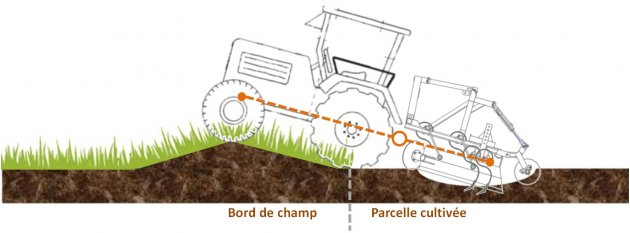
\includegraphics[width=0.9\columnwidth]{files/triangle_attelage_-_schema_sans_lumiere-52a8c}

\caption{Sans articulation}
\end{figure}


\begin{figure}[H]
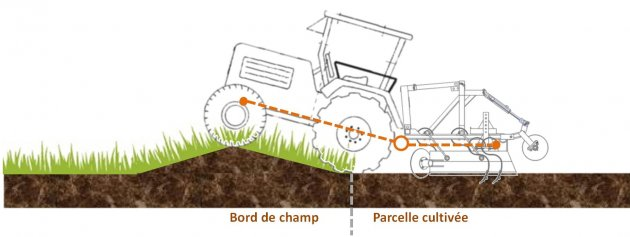
\includegraphics[width=0.9\columnwidth]{files/triangle_attelage_-_schema_avec_lumiere-9e61b}\caption{Avec articulation}
\end{figure}



\section*{Liens}

\href{http://www.adabio-autoconstruction.org/IMG/png/plan.png}{plans}

\href{http://www.adabio-autoconstruction.org/IMG/jpg/dscn0219_-_copie.jpg}{photo 1}

\href{http://www.adabio-autoconstruction.org/IMG/jpg/dscn0283_-_copie.jpg}{photo 2}

\href{http://www.dailymotion.com/video/xxm1em_fiche-outil-adabio-autoconstruction-bascule_tech\#.USM4kGfs-ZQ}{vidéo décrivant brièvement la construction}

\href{http://forum.adabio-autoconstruction.org/viewforum.php?f=56}{sujets concernant la bascule sur le forum.}
\end{document}
